С запада на восток Тайваня проходит большая железная дорога. Дорога разделена на $m$ зон.
Зоны пронумерованы $0, \ldots, m - 1$ с запада на восток. В каждой зоне есть два
параллельных пути~--- северный, по которому движение осуществляется с востока на запад, и
южный, по которому поезда движутся с запада на восток. В некоторых зонах расположена
железнодорожная станция.

Зоны могут быть трех различных типов. В зоне типа $C$ есть станция, к которой поезд может
подъехать по северному пути и выехать по южному. В зоне типа $D$ есть станция, к которой
поезд может подъехать по южному пути и выехать по северному. Кроме того, могут быть
пустые зоны, в которых нет железнодорожной станции.

Например, на рисунке ниже нулевая, четвертная и шестая зоны пустые, у первой, второй и
третьей зоны~--- тип $C$, а у пятой зоны~--- тип $D$. Зоны соединены друг с другом по прямой. Соответствующие пути соседних зон связаны друг с другом специальными соединительными устройствами, которые на рисунке изображены серыми прямоугольниками.

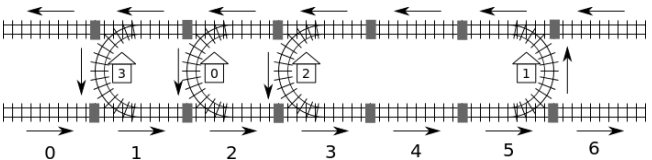
\includegraphics[scale=0.7]{1.png}

Железная дорога объединяет $n$ станций, пронумерованных от $0$ до $n - 1$. Будем считать,
что можно добраться от каждой станции до любой другой, используя железную дорогу.
Например, чтобы доехать от нулевой станции до второй, необходимо, начав движение из
второй зоны, проехать по южному пути через третью и четвертую зоны, проехать через пятую
зону, используя первую станцию, а потом по северному пути через четвертую зону доехать до
второй станции, расположенной в третьей зоне.

Так как от одной до другой станции существует несколько маршрутов, то расстояние от одной
до другой станции определяется как минимальное количество соединительных устройств,
которое необходимо проехать. Например, кратчайший маршрут от нулевой до второй станции
проходит через зоны $2-3-4-5-4-3$ и через пять соединительных устройств, то есть, расстояние
равно $5$.

Железными дорогами управляет автоматическая система. К сожалению, после внепланового
отключения электричества информация о расположении станций и типах зон была потеряна.
Однако, известно, что зона, в которой расположена нулевая станция, имеет тип $C$. К счастью, система умеет отвечать на запрос о расстоянии от станции до станции. Например, на запрос: <<Какое расстояние от станции $0$ до станции $2$?>>, система дает ответ $5$.

\textbf{Постановка задачи}

Вам необходимо реализовать функцию \texttt{findLocation}, которая определяет для каждой
станции номер зоны, в которой она находится, а также тип этой зоны.


\begin{itemize}
\item \texttt{void findLocation(int n, int first, int location[], int stype[])} 
\begin{itemize}
\item $n$: количество станций.
\item $first$: номер зоны, в которой расположена станция $0$.
\item $location$: массив размера $n$. Вы должны записать положение $i$-й станции в $location[i]$.
\item $stype$: массив размера $n$. Вы должно записать тип зоны, в которой расположена $i$-я станция в $stype[i]$. Используйте число $1$ для обозначения типа $C$, число $2$ для
обозначения типа $D$.
\end{itemize}
\end{itemize}

Для решения задачи вы можете использовать функцию \texttt{int getDistance(int i, int j)}.

\begin{itemize}
\item \texttt{getDistance(i, j)} возвращает расстояние от станции $i$ до станции $j$
\item \texttt{getDistance(i, i)} вернет $0$
\item \texttt{getDistance(i, j)} вернет $-1$ если $i$ или $j$ не удовлетворяет ограничениям $0 \le i, j \le n - 1$.
\end{itemize}
